\documentclass[tikz,border=2pt]{standalone}
\usepackage{amsmath,amssymb}
\usepackage{pgfplots}
\pgfplotsset{compat=1.18}
\usetikzlibrary{arrows.meta}
\begin{document}
% Loimaranta efficiency of the two-level one-year scheme b(lambda) = c(2 - e^{-lambda}):
% e(lambda) = lambda/(2e^lambda - 1), with e(0.5) ~ 0.2176 and maximum about 0.23; a proportional premium has e = 1.
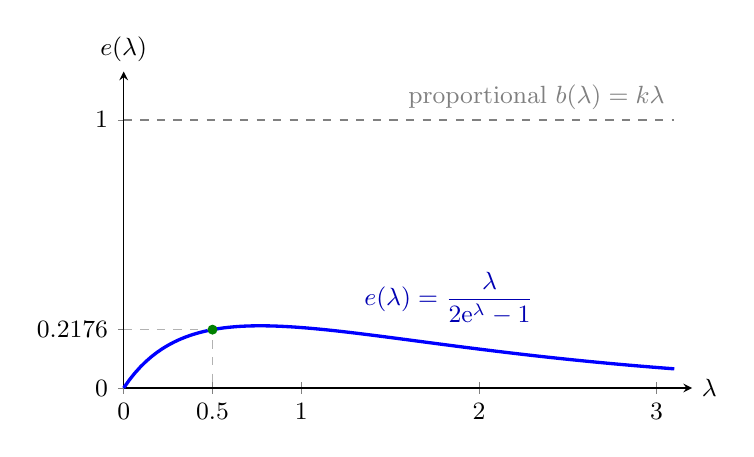
\begin{tikzpicture}[font=\small, >={Latex[length=2mm]}]
  \begin{axis}[
    axis lines=left, xmin=0, xmax=3.2, ymin=0, ymax=1.18,
    xtick={0,0.5,1,2,3}, ytick={0,0.2176,1}, yticklabels={$0$,$0.2176$,$1$},
    xlabel={$\lambda$}, ylabel={$e(\lambda)$},
    xlabel style={at={(axis description cs:1,0)}, anchor=west},
    ylabel style={rotate=-90, at={(axis description cs:0,1)}, anchor=south},
    width=8.8cm, height=5.6cm, clip=false
    ]
    \addplot[gray, thick, dashed, domain=0:3.1, samples=2] {1};
    \node[gray, anchor=south east] at (axis cs:3.1,1) {proportional $b(\lambda)=k\lambda$};
    \addplot[blue, very thick, domain=0:3.1, samples=100] {x/(2*exp(x)-1)};
    \draw[gray!60, thin, dashed] (axis cs:0,0.2176) -- (axis cs:0.5,0.2176) -- (axis cs:0.5,0);
    \fill[green!50!black] (axis cs:0.5,0.2176) circle (1.8pt);
    \node[blue!70!black, anchor=south west] at (axis cs:1.3,0.2) {$e(\lambda)=\dfrac{\lambda}{2\mathrm{e}^{\lambda}-1}$};
  \end{axis}
\end{tikzpicture}
\end{document}
